\documentclass[12pt,a4paper]{article}
\usepackage[utf8]{inputenc}
\usepackage[T1]{fontenc}
\usepackage{amsmath}
\usepackage{amsfonts}
%\usepackage{amssymb}
\usepackage{bbm}
\usepackage{graphicx}
\usepackage{geometry}
\usepackage{enumitem}
\usepackage{hyperref}

\usepackage{exsheets}
%\SetupExSheets{counter-format=qu}
\SetupExSheets{
  headings = block-subtitle ,
  headings-format = \normalsize\bfseries\sffamily ,
  % needs v0.16 2014/09/14 to work:
  subtitle-format = \normalsize\bfseries\sffamily
}

\SetupExSheets{
  counter-within = section ,
  counter-format = se.qu\IfQuestionSubtitleT{:} ,
}

\geometry{a4paper, margin=2cm}

\usepackage{cprotect}

\usepackage{xcolor}
\definecolor{maroon}{cmyk}{0, 0.87, 0.68, 0.32}
\definecolor{halfgray}{gray}{0.55}
\definecolor{ipython-frame}{RGB}{207, 207, 207}
\definecolor{ipython-bg}{RGB}{247, 247, 247}
\definecolor{ipython-red}{RGB}{186, 33, 33}
\definecolor{ipython-green}{RGB}{0, 200, 0}
\definecolor{ipython-cyan}{RGB}{64, 128, 128}
\definecolor{ipython-purple}{RGB}{170, 34, 255}

\usepackage{listings}
\lstdefinelanguage{iPython}{
	morekeywords={access,and,del,except,exec,in,is,lambda,not,or,raise},
	morekeywords=[2]{for,print,abs,all,any,basestring,bin,bool,bytearray,callable,chr,classmethod,cmp,compile,complex,delattr,dict,dir,divmod,enumerate,eval,execfile,file,filter,float,format,frozenset,getattr,globals,hasattr,hash,help,hex,id,input,int,isinstance,issubclass,iter,len,list,locals,long,map,max,memoryview,min,next,object,oct,open,ord,pow,property,range,reduce,reload,repr,reversed,round,set,setattr,slice,sorted,staticmethod,str,sum,super,tuple,type,unichr,unicode,vars,xrange,zip,apply,buffer,coerce,intern,elif,else,if,continue,break,while,class,def,return,try,except,import,finally,try,except,from,global,pass, True, False},
	sensitive=true,
	morecomment=[l]\#,%
	morestring=[b]',%
	morestring=[b]",%
	moredelim=**[is][\color{black}]{@@}{@@},
	identifierstyle=\color{black}\footnotesize\ttfamily,
	commentstyle=\color{ipython-cyan}\footnotesize\itshape\ttfamily,
	stringstyle=\color{ipython-red}\footnotesize\ttfamily,
	keepspaces=true,
	showspaces=false,
	showstringspaces=false,
	rulecolor=\color{ipython-frame},
	frame=single,
	frameround={t}{t}{t}{t},
	backgroundcolor=\color{ipython-bg},
	basicstyle=\footnotesize\ttfamily,
	keywordstyle=[2]\color{ipython-green}\bfseries\footnotesize\ttfamily, 
	keywordstyle=\color{ipython-purple}\bfseries\footnotesize\ttfamily
}

\lstdefinelanguage{iOutput} {
	sensitive=true,
	identifierstyle=\color{black}\small\ttfamily,
	stringstyle=\color{ipython-red}\small\ttfamily,
	keepspaces=true,
	showspaces=false,
	showstringspaces=false,
	rulecolor=\color{ipython-frame},
	basicstyle=\small\ttfamily,
}

\lstnewenvironment{ipython}[1][]{\lstset{language=iPython,mathescape=true,escapeinside={*@}{@*}}%
}{%
}

\lstnewenvironment{ioutput}[1][]{\lstset{language=iOutput,mathescape=true,escapeinside={*@}{@*}}%
}{%
}

\newcommand{\myendproof}{\hfill\qedsymbol}

\title{Addons with Python Exercises}
\author{Matteo Sani}

\begin{document}
\maketitle

\section{Stochastic Simulation}
In science, we are often more interested in the distribution of a set of outcomes rather than a single event. This may be the probability distribution of a molecule diffusing a specific distance as a function of time, or the price change of a very exotic derivative.

Stochastic simulations allow us to generate a series of experiments on a system in which one step is governed by random chance. These simulations often boil down to flipping a coin to dictate if said step will occur or not.

Of course, sitting in your office chair flipping a coin over and over again is not how one should do a simulation. To get a sense of the probability distribution of some outcome, we often have to simulate the process thousands of times. This means that we need to know how to make our computers do the heavy lifting.

It's often easy to forget just how powerful modern computers can be. What once required a serious computational cluster only twenty years ago can now be done on a 10 mm thick compartment made of rose-gold colored aluminium. 

%FIXME few words about mean and C.L.

\begin{question}
Using a Monte Carlo simulation of coin flip demonstrate the Central Limit Theorem.
\end{question}

\subsection{1D Random Walk}
The Random Walk in one dimension is a model for each process which have simple binary outcomes.

The 1D random walk can be used to model how a gambler plays a game such as roulette in a casino. The idea in such games is that the gambler places a small stake on each game (say 1€). When the game is played the gambler will either loose and the total amount of money he has will thus decrease by one unit, or alternatively, he will win the game and in that case he wins back his stake and a prize, which we will set as 1€. As you can see if the gambler repeats this process of staking money and playing the amount of money he has will undergo a random walk in one dimension, since the outcome will be either 1 or -1.

\begin{question}
Code a function that simulate a 1D random walk. 

\noindent
\textbf{Hint:} we can decide whether to walk left or right by flipping a coin and seeing if it comes up \emph{heads} or \emph{tails}.
\end{question}

\subsubsection{Simulating a Gambler}

Importantly there is a difference between the gambler and the 1D random walk, however. The gambler usually only has a finite amount of money to gamble with. If he looses a large number of games he is therefore forced to stop playing. Similarly, the gambler may also have some target for how much money he would like to win. In other words, he should have some figure $N$€, which is more than the amount of money he entered the casino with. He will stop gambling once he has $N$€ in his pocket.

\begin{question}
Determine with a simulation the probabilities whether the gambler leaves the casino with zero or with $N$€.

Essentially we start the gambler with $X$€ and simulate the process of him playing the game only stopping once he has reached one of the two thresholds.

Write a function called gambler that simulates this procedure, taking three arguments:
\begin{itemize}
\item \texttt{start}: the amount of money the gambler starts with; \item \texttt{n}: the target amount of money that the gambler wants to win;
\item \texttt{p}: the probability of winning each individual game the gambler plays.
\end{itemize}
\end{question}

We can also use simulation to determine how many spins of the wheel the gambler will play before leaving the casino (i.e. \emph{hitting time}).
In other words we want to calculate the number of steps the random walk takes before arriving in one of the two threshold states.

\begin{question}
Write another function that simulates the changes in the amount of money the gambler has and that returns the number of spins of the wheel that take place.
\end{question}

\subsection{Martingale Examples}
Suppose you play the following series of games. In game $i, i = 1, 2,\ldots$, you bet \$1 and roll a fair die. If the outcome is $\{1,2\}$ you win \$1, if it is $\{3,4\}$ nothing happens, and if the outcome is $\{5,6\}$ you lose \$1.
Let $X_i$ be a random variable representing the amount of money you win or lose in bet $i$, this kind of game is said to be **fair** since

$$\mathbb{E}[X_i]= \sum_{\Omega}p(\omega)\cdot x(\omega) = \frac{2}{6}\cdot 1 + \frac{2}{6}\cdot 0 + \frac{2}{6}\cdot -1 = 0\;\forall i$$
so no unbalance between losses or wins.

Now define another random variable $Z_n = \sum_{i=1}^{n} X_i$, i.e. the amount of money held at the $n$-th game.

$Z_n$ is a martingale and $\mathbb{E}[Z_n|X_1,\ldots, X_{n-1}] = Z_{n-1}$.

\paragraph{Proof}

\begin{equation*}
	\begin{aligned}
		\mathbb{E}[Z_n|X_1,\ldots, X_{n-1}] &= \mathbb{E}[X_1 +\ldots + X_n|X_1,\ldots, X_{n-1}] \\
		& = \underbrace{\mathbb{E}[X_1|X_1,\ldots, X_{n-1}]}_{X_1} + \ldots + \underbrace{\mathbb{E}[X_{n-1}|X_1,\ldots, X_{n-1}]}_{X_{n-1}} + \underbrace{\mathbb{E}[X_n|X_1,\ldots, X_{n-1}]}_{\mathbb{E}[X_n]=0} \\
		& = \mathbb{E}[X_1|X_1,\ldots, X_{n-1}] + \ldots + \mathbb{E}[X_{n-1}|X_1,\ldots, X_{n-1}] + 0 = Z_{n-1}
	\end{aligned}
\end{equation*}

\begin{question}
Using Monte Carlo simulation implement the game described in the text and check that the expected gain is indeed null.
\end{question}

\begin{question}
An unbiased random walk (in any number of dimensions) is another example of a martingale.

In higher dimensions, the set of randomly walked points has interesting geometric properties. In fact, one gets a discrete \emph{fractal}, that is, a set that exhibits stochastic self-similarity on large scales.

Implement a 2D random walk simulation and plot one possible realization.
\end{question}

\subsection{Simulating Stochastic Differential Equations}

Consider a generic stochastic differential equation (SDE)

\begin{equation}
dX(t) = \mu(t,X(t))dt + \sigma(t,X(t))dW(t)
\label{eq:sde}
\end{equation}

The Monte Carlo simulation of such a process can be carried out according to the \emph{Euler scheme} as follows: consider the value of $X$ at time $t=t_i$, the value compute $X(t_{i+1})$ is evaluated from the dynamics of X (Eq.~\ref{eq:sde}), setting $\Delta t = t_{i+1} - t_{i}$, and sampling from a standard normal $\mathcal{N}(0,1)$ in order to "evolve" the stochastic term $dW$
\begin{equation}
X(t_{i+1}) = X(t_i) + \mu(t_i,X(t_i))\Delta t + \sigma(t_i,X(t_i))\sqrt{\Delta t}\mathcal{N}(0,1)
\end{equation}

In the specific case of a simple Brownian motion the dynamics is given by
\begin{equation}
dW = \sqrt{dt}\mathcal{N}(0,1)
\end{equation}
so
\begin{equation}
W(t+dt) = W(t) + \sqrt{dt}\mathcal{N}(0,1)
\end{equation}
or
\begin{equation}
W(t) = \sum_{t_0}^{t} \sqrt{dt}\mathcal{N}(0,1)
\end{equation}

\begin{question}
Simulate a couple of realization of a Brownian motion process with initial value 0.
Figure~\ref{fig:brownian_motion} reports two realization of the Brownian motion simulated according to the Euler scheme.

\begin{figure}[htbp]
\begin{center}
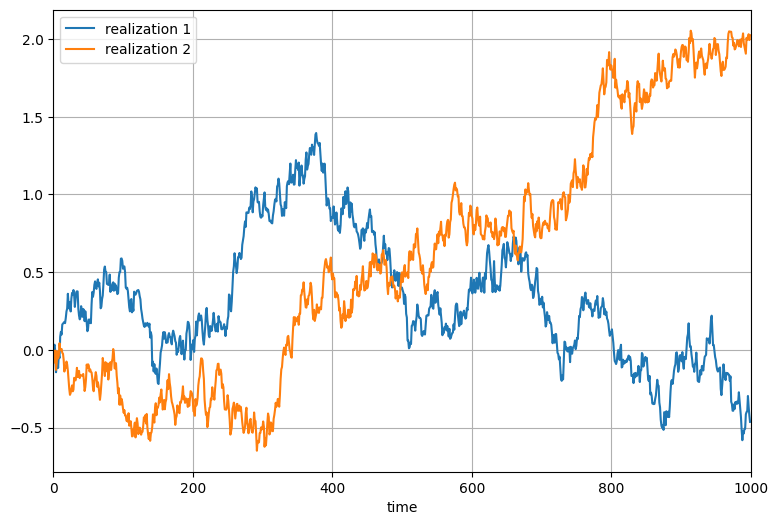
\includegraphics[width=0.5\linewidth]{addons/brownian_motion}
\end{center}
\label{fig:brownian_motion}
\end{figure}
\end{question}

\begin{question}
Using the Euler scheme simulate the 4-months (with daily steps) evolution of a Geometric Brownian Motion stochastic process with initial value $S_0=100$, $\mu=0.005$, and $\sigma=0.05$.
\end{question}

\cprotEnv\begin{question}
This \href{https://github.com/matteosan1/advanced_financial_modeling/raw/master/input_files}{file} contains a thousand 10-day realizations (with 0.1 day step) of historical price data of a single asset, assume that all the time series are different realizations of the same stochastic process.
\begin{enumerate}
\item Make two figures: the first should contain one realization as a function of time, in the second plot the first 50 realizations together as a function of time (\emph{label the axes appropriately}).
\item In two separated plots report the mean and the variance of the stock prices as a function of time (\emph{label the axes appropriately}).
\item Perform the variable change $X_{n+1}=\log\left(\cfrac{S_{n+1}}{S_n}\right)$ on $S_{n+1} = S_ne^{(\mu-0.5\sigma^2)\Delta t + \sigma\sqrt{\Delta t}Z}$ to rewrite the model into a simpler form. 
	\begin{enumerate}
	\item Is the resulting dynamics linear ? Prove it, or give a counterexample; 
	\item is the resulting system time-invariant ? Prove it, or give a counterexample.
	\end{enumerate}
\item Apply again the same transformation $X_{n+1}=\log\left(\frac{S_{n+1}}{S_n}\right)$ to data this time. Plot both the mean and the variance of the transformed realizations as a function of time.
\end{enumerate}

\noindent
\textbf{Hint:} the input file is a binary file that can be loaded back using \texttt{numpy} as follows (replace the URL from the link above):
\begin{ipython}
import numpy as np

path = np.DataSource("https://github.com/matteosan1/...../input_files")
S = np.load(path.open("stock_2023.npy", "rb"))
\end{ipython}
\end{question}

\begin{question}
The Heston model can be considered an extension of the Black and Scholes model where the volatility of the underlying asset is not constant, nor even deterministic, but follows a random process.

The basic Heston model assumes that $S_t$, the price of the asset, follows
\begin{equation}
dS_{t}=\mu S_{t}\,dt+{\sqrt {\nu _{t}}}S_{t}\,dW_{t}^{S}
\end{equation}
where the volatility 
\begin{equation}
{\displaystyle d\nu _{t}=\kappa (\theta -\nu _{t})\,dt+\xi {\sqrt {\nu _{t}}}\,dW_{t}^{\nu },}
\end{equation}
and 
\begin{equation}
W_{t}^{S},W_{t}^{\nu }
\end{equation} 
are Wiener processes with correlation $\rho$.

The model has five parameters:
\begin{itemize}
\item $\nu _0$, the initial variance;
\item $\theta$, the long variance of the price; as $t$ tends to infinity, the expected value of $\nu_t$ tends to $\theta$;
\item $\rho$, the correlation of the two Wiener processes;
\item $\kappa$, the rate at which $\nu_t$ reverts to $\theta$;
\item $\xi$, the volatility of the volatility, which determines the variance of $\nu_t$.
\end{itemize}

Using the Euler scheme simulate a possible realization for $S_t$ and $\sigma_t$ using the parameters: $S_0=100$, $\mu=0.25$, $T=3$, $\nu_0=0.05$, $\kappa=1.2$, $\theta=0.10$, $\xi=0.593$, $\rho=-0.5$.

\begin{figure}[htbp]
\begin{center}
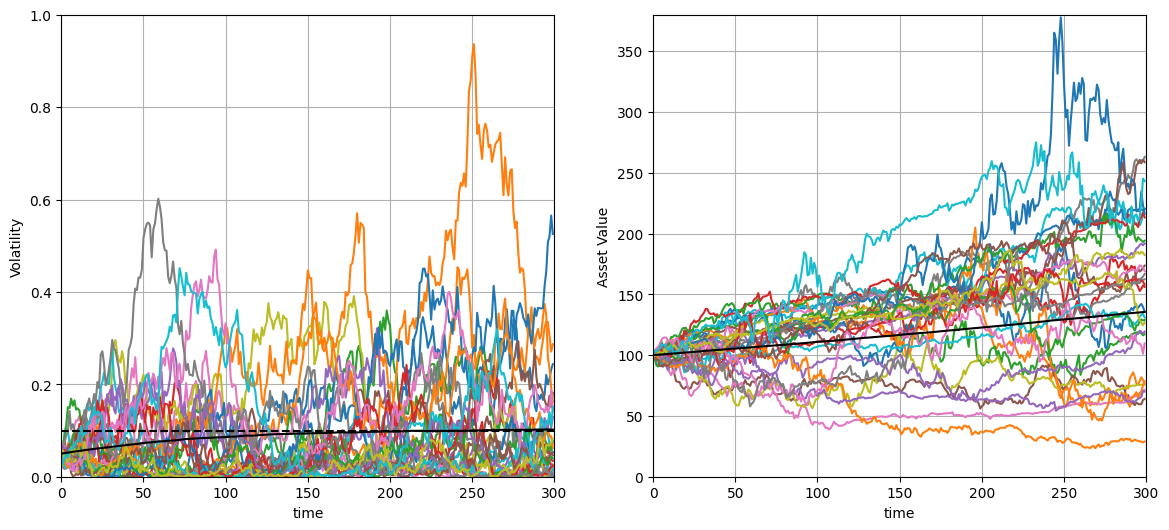
\includegraphics[width=0.8\linewidth]{addons/heston}
\end{center}
\label{fig:heston}
\end{figure}
\end{question}

\begin{question}
Using the Euler scheme simulate few realization from a short rate process following the Hull and White model.
\end{question}

\clearpage

\section{Forward Rate Agreement}
Below is presented yet another alternative methods to determine the valuation formula for forward rate agreement.

\subsection{Valuation by Replication}
Let's try to estimate the value of a FRA using a simple replication approach:
\begin{itemize}
\item at time $t$: 
	\begin{equation*}
	\begin{cases}
		\text{lend}~P(t,T)\\
		\text{borrow}~P(t,S)(1+\tau(T,S)K)
	\end{cases};
	\end{equation*}
\item at time $T$: you receive 1 which you will invest at the (in $t$ unknown) EURIBOR rate $L(T,S)$;
\item at time $S$: 
	\begin{equation*}
		\begin{cases}
			\text{receive}~(1+L(T,S)\tau(T,S))\\
			\text{pay}~1 + \tau(T,S)K
		\end{cases}.
	\end{equation*}
\end{itemize}

Adding the cash-flows together and evaluating in $t$ we get:
\begin{equation*}
	1+L(T,S)\tau - 1 - \tau K = (L(T,S)-K)\tau
\end{equation*}
From the risk-neutral pricing formula
	\begin{equation*}
		\mathbb{E}^Q[D(t, S)(L(T, S)-K)\tau(T,S)|\mathcal{F}_t]
	\end{equation*}
but according to the \emph{Fundamental Theorem of Pricing II} its value must equal the value of the replicating portfolio in $t$ (we assume to be in a complete market). Hence
\begin{equation}
	\begin{aligned}
		\mathbb{E}^Q[D(t,S)&(L(T,S)-K)\tau(T,S)|\mathcal{F}_t]=\\
			&[P(t,S)\tau(T,S)K-P(t,T)+P(t,S)]
			\label{eq:fra_as_expectation}
	\end{aligned}
%	\myendproof
\end{equation}

%\subsection{Forward Rate and No-Arbitrage Approach}
%Following Filipovic (2009) we can define the Forward Rate by implementing the following:
%		\item at time $t$
%		\begin{equation*}
%			\begin{cases}
%				\text{sell one $T$-ZCB}\\
%				\text{buy $\frac{P(t,T)}{P(t,S)}$ $S$-ZCB}\\
%			\end{cases} 
%		\end{equation*}
%		which results in a zero net investment;
%		\item at $T$ you must pay 1;
%		\item at time $S$ you receive $\frac{P(t,T)}{P(t,S)}$;
%		\item the net effect of the operation is a \emph{forward} investment of one dollar a time $T$ yielding $\frac{P(t,T)}{P(t,S)}$ so
%		\begin{equation*}
%			1 + \tau(T,S)F(t;T,S) = \frac{P(t,T)}{P(t,S)}
%		\end{equation*}
%	%	\myendproof
%	\end{itemize}

\clearpage
\section{Interest Rate Swap as FRAs}

The swap payoff 

\begin{equation}
	\sum_{i=\alpha+1}^{\beta} D(t,T_i)N \tau_i \left[K-L(T_{i-1},T_i)\right]
	\label{eq:payoff_payer_irs}
\end{equation}	
can be re-interpreted as a portfolio of FRAs. Indeed using the payoff of a FRA
\begin{equation}
	\textbf{FRA}= N\tau P(t,S)(K - F(t;T,S))
	\label{eq:fram_payoff_withF}
\end{equation}
the Receiver IRS payoff can be expressed like
\begin{equation}
	\begin{aligned}
		\textbf{RFS}&(t,T,\tau,N,K) = 	N\sum_{i=\alpha+1}^{\beta}\mathbb{E}^Q[D(t,S)\tau_i(K - L(T_{i-1},T_i))]=\\
		&=N\sum_{i=\alpha+1}^{\beta}\tau_i P(t,T_i)(K-F(t;T_{i-1},T_i))\\
		&=N\sum_{i=\alpha+1}^{\beta}\tau_i KP(t,T_i)-N\sum_{i=\alpha+1}^{\beta}(P(t,T_{i-1})-P(t,T_i)) \\
		&=N\sum_{i=\alpha+1}^{\beta}\tau_i KP(t,T_i)-NP(t,T_\alpha)+NP(t,T_\beta)
	\end{aligned}
\label{eq:swap_as_sum_fra}
\end{equation}

Clearly not all the FRAs in the swap, when it has zero value, will have zero value each (\emph{except for the degenerate case of flat yield curve}): some of them will have positive NPV, some other negative; the only constraint being their sum to be zero.

\begin{question}
Implementing a class or a function that represents an interest rate swap shows that:
\begin{enumerate}
\item In a \emph{Payer Swap} with an increasing yield curve the first FRAs will have negative value, the last positive. 
\item In a \emph{Payer Swap} with a decreasing yield curve the first FRAs will have positive value, the last negative.
\end{enumerate}
\end{question}

\clearpage
\section{Floating Rate Notes}
Floating rate bond or note (FRN) usually refers to an instrument whose coupon is based on a short term rate (3-month T-bill, 6-month LIBOR). Variable coupon rates are fixed in advance at reset dates, which are 3- or 6-month (interest payment period) earlier.

In this example we use an annual payment frequency but the extension to the quarterly or semi-annual frequency is straightforward.

Floating rate bond price with (\emph{unit notional amount}), $n$ maturity, annual frequency ($\tau=1$), and the first coupon rate predetermined at previous reset date ($C_{reset}$) is as follows.

\begin{equation}
	\begin{aligned}
		\textbf{FRN} & = D_{0,1}C_{reset} + \sum_{i=1}^nD_{0,i}f_{i,i+1} + D_{0,n}= \\
		& = D_{0,1}C_{reset} + D_{0,2}f_{1,2} + \ldots + D_{0,n-1}f_{n-2,n-1}+ D_{0,n}(1+f_{n-1,n}) = \\
		& = D_{0,1}C_{reset} + D_{0,2}\left(\frac{D_{0,1}}{D_{0,2}}-1\right) + \ldots \\
		&\quad\ldots + D_{0,n-1}\left(\frac{D_{0,n-2}}{D_{0,n-1}}-1\right) + D_{0,n}\left(\frac{D_{0,n-1}}{D_{0,n}}-1\right) + D_{0,n} = \\
		& = D_{0,1}C_{reset} + (D_{0,1} - D_{0,2}) + (D_{0,2} - D_{0,3}) + \ldots \\
		&\quad\ldots + (D_{0,n-2} - D_{0,n-1}) + (D_{0,n-1} - D_{0,n}) + D_{0,n} = \boxed{D_{0,1} (1 +C_{reset})}
	\end{aligned}
\end{equation}
where $f(t_1,t_2)$ denotes the forward rate between $t_1$ and $t_2$.

If the remaining maturity of the above \textbf{FRN} for example was 4.25 year, its price will be
\begin{equation}
	\textbf{FRN} = D_{0,\frac{1}{4}}(1+C_{reset})
\end{equation}

If the remaining maturity of the above \textbf{FRN} was $(4 + \epsilon)$ year, in this case, the price would be

\begin{equation}
	\begin{aligned}
		\textbf{FRN} &= D_{0,1}f_{0,1}+ D_{0,2}f_{1,2} + \ldots + D_{0,n-1}f_{n-2,n-1} + D_{0,n}(1+f_{n-1,n}) = \\
		& = D_{0,1}\left(\frac{D_{0,0}}{D_{0,1}}-1\right) + D_{0,2}\left(\frac{D_{0,1}}{D_{0,2}}-1\right) + \ldots \\
		&\quad\ldots + D_{0,n-1}\left(\frac{D_{0,n-2}}{D_{0,n-1}}-1\right) + D_{0,n}\left(\frac{D_{0,n-1}}{D_{0,n}}-1\right) + D_{0,n} = \\
		&= (D_{0,0}-D_{0,1})+(D_{0,1}-D_{0,2}) + \ldots \\
		&\quad\ldots + (D_{0,n-2}-D_{0,n-1})+(D_{0,n-1}-D_{0,n})+D_{0,n} = 1
	\end{aligned}
\end{equation}

The price of FRN has a range from \emph{par} to \emph{par} + full coupon. It is par right before the reset date and is $C$ right after the reset date (and is linear when pricing date is between two reset dates).

\begin{question}
	Draw a plot showing the characteristic sawtooth behaviour of a floating rate note. The relevant insterest rates can be taken from \href{https://raw.githubusercontent.com/matteosan1/advanced\_financial\_modeling/master/input_files/libor.csv}{libor.csv}
	
	\begin{center}
		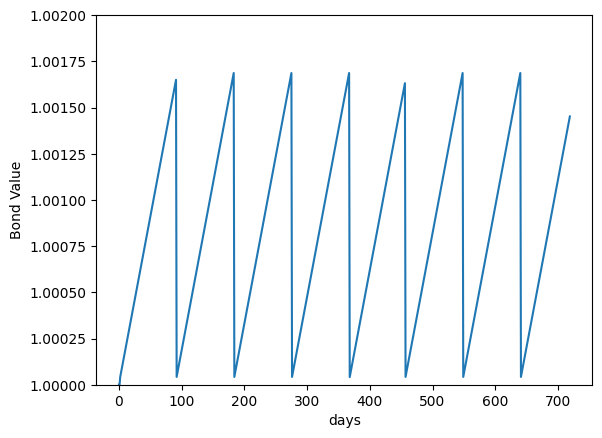
\includegraphics[width=0.6\linewidth]{addons/floating_rate_note}
	\end{center}
\end{question}
\clearpage

\section{Asset Swap}

The underlying bond in the asset swap package is credit risky and can default. The bond purchaser’s claim is on the recovery value of the bond, however she must continue to honor the bond coupons on the swap (of course she may choose to close the swap position at market value). The asset swap seller is therefore taking on this credit risk, which could be hedged with Credit Default Swaps.

Many bonds do not have a liquid CDS market and even when they do the trader often cannot match the hedge to the maturity of the asset swap, since often only the 5Y CDS contracts are liquid. Often credit risk is hedged using a proxy bond issuer or CDS reference entity, whereby we receive a protection or insurance payout if a highly correlated credit defaults, but we don’t receive a credit protection on the exact same bond issuer referenced in our asset swap.

%Finally we should also note that in the event of a default we receive a payout to cover losses on our bond notional, but we are not compensated for losses on the bond coupons themselves.
Suffice to say if and when traders purchase credit protection using CDS contracts this does not typically provide a perfect hedge and we carry some residual credit risk or credit basis risk.

Asset swaps are quoted in the market as a spread, which incorporates both funding costs and a premium for credit protection. The spread attempts to make the swap in some way equivalent to a bond.

The bonds of issuers of good credit quality, of some governments such as Germany and good quality government agency bonds trade at negative spreads to swaps, and especially so for the shorter maturity bonds. The opposite is true for poor or low quality credits such as Greek and Argentina sovereigns and many corporate bonds, which trade with positive spreads. For good quality credits a widening of the spread, which is negative, refers to a richening of the bond (decline in bond yield relative to swaps) and for poor quality credits the opposite is true, namely a widening of the positive spread reflects a cheapening of the bond and increase in bond yield.

\begin{question}
Consider a 1Y risky bond paying quarterly coupons. The bond issuer has a default probability of 5\% during the next year. The interest rate term structure is considered flat at 0.05.

\begin{itemize}
\item If the bond buyer enters into an asset swap, determine its spread;
\item check that a CDS with same maturity as the asset swap has similar spread;
\item finally check how the spread change as a function of the probability of default.
\end{itemize}
\begin{center}
	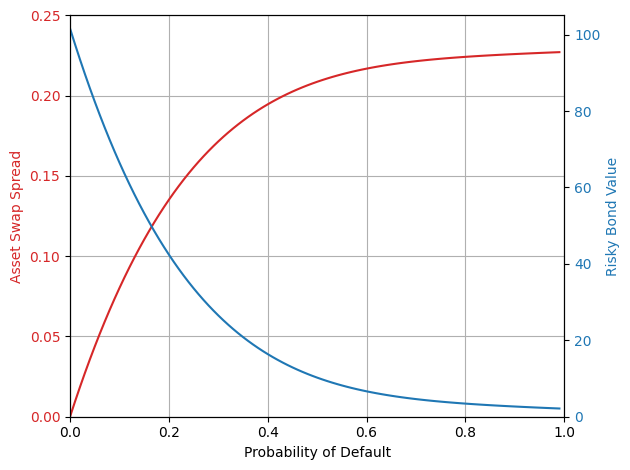
\includegraphics[width=0.6\linewidth]{addons/asset_swap_spread}
\end{center}
\end{question}

\begin{question}
	Consider the 10-year German Bund DBR 0.5\% 2026 which is currently trading at a clean price of 104.58. 
	Given that the 10-year EUR swap rate is 0.44\% what is the par-par asset swap spread for this bond? 
	For this exercise assume the all Annuity Factors have a value of 10.0 for simplicity.
\end{question}
Recall the Asset Swap Spread $s$ can be calculated using 
Firstly we calculate the swap components giving 
The Par-Par adjustment is the dominating term and evaluates to
Par-Par Adjustment =

%100 − 104.58
%100 !
%= -4.580%
%We proceed to calculate the asset swap spread s as
%s =
%0.600% - 4.580%
%10.0
%= -0.3980%
%or -39.80 basis points
%
%Consider the 10-year Greek Government Bond GGB 3.0\% 2026 which is currently trading at a clean price of 75.280. Given that the 10-year EUR swap rate is 0.440\% what
%is the par-par asset swap spread for this bond?
%Using the Asset Swap Spread $s$ can be calculated using 
%Again we calculate the swap components giving
%The Par-Par adjustment evaluates to
%Par-Par Adjustment =
%
%100 - 75.280
%100 !
%= 24.72%
%We proceed to calculate the asset swap spread s as
%s =
%25.60% + 24.72%
%10.0
%= 5.0320%
%or 503.20 basis points

\clearpage
\section{Algorithmic Differentiation}

\emph{Algorithmic Differentiation} (AD), also known as \emph{automatic differentiation}, is a mathematical, computer science technique for computing accurate sensitivities quickly. There are two main modes, namely \textbf{tangent mode} and \text{adjoint mode}. For many models, \emph{adjoint AD (AAD)} can compute sensitivities from to 10x to 1000x faster than numerical bumping or finite differences. AD operates directly on analytics and each line of code is differentiated. Clearly it can be applied to a single trade or a portfolio (or vector) of trades.

If for example we have a computer algorithm that computes $y$ via multiple nested operations such as $y = h(g(f(x)))$ we could illustrate the series of operations as,
\begin{equation}
x\rightarrow f(x) \rightarrow g(f(x)) \rightarrow h(g(f(x))) \rightarrow y
\end{equation}

Working forwards from the input value $x$, we can compute the derivative of each operation and use the \emph{chain rule} to compute the total derivative $dy/dx$ as follows
\begin{equation}
\frac{df}{dx}\frac{dg}{df}\frac{dh}{dg}\frac{dy}{dh}=\frac{dy}{dx}
\end{equation}
But in principle we could also work backwards, from the output value $y$ to arrive at the same result,
\begin{equation}
\frac{dy}{dh}\frac{dh}{dg}\frac{dg}{df}\frac{df}{dx}=\frac{dy}{dx}
\end{equation}
Furthermore AD can be used on systems of equations and matrices. 
Tangent mode works forward from the left to right
\begin{equation}
\left(\left(\left(\frac{\partial x_1}{\partial x}\frac{\partial x_2}{\partial x_1}\right)\frac{\partial x_3}{\partial x_2}\right)\cdots\frac{\partial x_m}{\partial x_{m-1}}\right)\frac{\partial y}{\partial x_m}
\end{equation}
With adjoint mode we work backwards from the right
\begin{equation}
\frac{\partial x_1}{\partial x}\left(\frac{\partial x_2}{\partial x_2}\left(\frac{\partial x_3}{\partial x_2}\cdots\left(\frac{\partial x_m}{\partial x_{m-1}}\frac{\partial y}{\partial x_m}\right)\right)\right)
\end{equation}

\subsection{Tangent Mode}
In tangent mode we differentiate code working forwards starting with the trade inputs and follow the natural order of the original program. This method computes price sensitivities to one input at a time and we must call the tangent method several times, once for each input parameter.

When using tangent mode \emph{dot} notation is usually used to denote derivatives being differentiated with respect to the function input. For example given $y = f(x)$ then $y$ dot would indicate $\dot{y} = dy/dx$.
Consider the below simple function,
\begin{equation}
\begin{cases}
\text{Function: } y = 2x^2\\
\text{Tangent: } \dot{y} = 4x\dot{x}
\end{cases}
\label{eq:aad_function}
\end{equation}
In tangent mode $\dot{x}=dx/dx$ is specified as an input and used to enable/disable the tangent derivative calculation. Setting it to 1 in enables the derivative calculation giving
$dy/dx = 4x$, however when $\dot{x}= 0$ we have $dy/dx = 0$.

\subsection{Adjoint Mode}
When using adjoint mode we differentiate code in reverse order, starting with function outputs. 
Adjoint mode follows the reverse order of the original program, consequently we must compute the function value first (\emph{forward sweep}) and store the intermediate values before applying adjoint AD in reverse (\emph{back propagation}). This method shifts one function output at a time and generates derivatives exactly to machine precision for all price inputs in one go.

Adjoint mode is computed using \emph{bar} notation for derivatives to denote the variable is to be differentiated with respect to the function input. For example given $y = f(x)$ and working in reverse order gives $\bar{y} = dy/dx$
Once again let us consider same simple function from before,
\begin{equation}
\begin{cases}
\text{Function: } y = 2x^2\\
\text{Tangent: } \bar{y} = 4x\bar{x}
\end{cases}
\end{equation}
In adjoint mode $\bar{y} = dy/dy$ is specified as an input and allows us to enable/disable the adjoint derivative calculation. 

\begin{question}
Consider the function define in Eq.~\ref{eq:aad_function} and compute the AD both using tangent and adjoint technique.
\begin{equation}
\begin{cases}
\text{Function: } f(x_1, x_2) = 2x_1^2 + 3x_2\\
\text{Solution: } \frac{df}{dx_1} = 4x_1, \text{ and } \frac{df}{dx_2}=3
\end{cases}
\end{equation}
When for example $x_1=2$ and $x_2 = 3$ we have,
\begin{equation}
\frac{df}{dx_1} = 8, \text{ and } \frac{df}{dx_2}=3
\end{equation}
\end{question}

\begin{question}
Consider a 5-years receiver Interest Rate Swap with a 1M notional, exchanging a fixed rate of 5\% with a flat 1\% LIBOR rate. The risk free rate for discounting is considered to be flat a 1.5\%.
Compute DV01 and PV01 with algorithmic differentiation using both tangent and adjoint modes. Compare the results.
\end{question}
\clearpage

\section{Newton-Raphson Method}
Newton's method, also known as the Newton–Raphson method, is a root-finding algorithm which produces successively better approximations to the roots (or zeroes) of a real-valued function. %The most basic version starts with a real-valued function f, its derivative f′, and an initial guess x0 for a root of f. If f satisfies certain assumptions and the initial guess is close, then

The idea is to start with an initial guess, then to approximate the function by its tangent line, and finally to compute the $x$-intercept of this tangent line. This $x$-intercept will typically be a better approximation to the original function's root than the first guess, and the method can be iterated.

If the tangent line to the curve $f(x)$ at $x = x_n$ intercepts the $x$-axis at $x_{n+1}$ then the slope is
\begin{equation}
	f'(x_n)=\dfrac {f(x_{n})-0}{x_{n}-x_{n+1}}
\end{equation}

Solving for $x_{n+1}$ gives
\begin{equation}
	x_{n+1}=x_{n}-{\frac {f(x_{n})}{f'(x_{n})}}
\end{equation}

We start the process with some arbitrary initial value $x_0$ (the closer to the zero, the better). The method will usually converge, provided this initial guess is close enough to the unknown zero, and that $f'(x_0) \neq 0$.
\begin{center}
	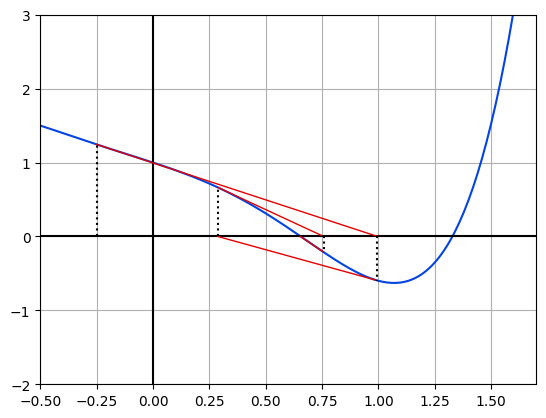
\includegraphics[width=0.6\linewidth]{addons/newton_method}
\end{center}

\clearpage

\section{Bootstrap}

\emph{Bootstrap} is an algorithm that allows to determine a vector of values that are implicitly defined by a set of equations.

Consider the following system 
\begin{equation}
	\begin{cases}
		f_1(x_1, c) = 0\\
		f_2(x_1, x_2, c) = 0\\
		f_3(x_1, x_2, x_3, c) = 0\\
		\vdots
		f_n(x_1,\ldots,x_n, c) = 0\\
	\end{cases}
\label{eq:bootstrap}
\end{equation}
It is possible to find the vector $\bar{x} = \{x_1,\ldots,x_n\}$ which simultaneously satisfy all the equation in~\ref{eq:bootstrap}, with an iterative algorithm as follows.
Indeed, solving the first equation, either analytically or numerically, we get $x_1 = f_1^{-1}(c)$ that can be used to solve the second equation as $x_2 = f_2^{-1}(x_1, c)$.
Going on, \emph{iteratively}, through each equation we are then able to determine all the unknown $\bar{X}$ values.

As a financial example, you can imagine the functions $f_i$ as the pricing equation of bonds with different maturities, each depending on a different set of interest rates, minus the current market price of the bond $c$. Since those are fair prices each $f_i$ can be set equal to 0 and through the bootstrap we can determine the interest rate term-structure implied by the bond market quotes. 

\subsection{Cap Volatilities}

Another practical application of the bootstrap algorithm is to determine the \emph{spot cap volatilities} from the current market prices (note, the market quotes only the flat volatilities).

The main challenges are:
\begin{enumerate}
	\item Produce Caplet/Floorlet prices consistent with current levels of Cap/Floor volatilities and therefore be able to re-price the market;
	\item being able to “rebase” volatilities when pricing Cap/Floor over not quoted floating rates according to multiple curves framework (e.g. Cap/Floor over 1M or 12M Euribor);
	\item to make things more complicated, some Caps/Floors are not always quoted over the same LIBOR, for example EUR Cap/Floor are quoted over 3M EURIBOR up to $2y$ maturity and then over 6M EURIBOR.
\end{enumerate}

From the prices of different maturity caps, it is possible to \emph{bootstrap} the volatility of each caplet, i.e. the volatility which refers to the forward rate corresponding to the caplet.

\begin{question}
Given the following set of flat volatilities use the bootstrap algorithm to determine the implied spot volatilities.

Let's \emph{strip} caplet volatilities from the following cap (flat) volatilities which refers to caps with 0.013 strike over EURIBOR-6M whose term structure is shown in Table~\ref{tab:flat_volatilities}(right).

\begin{table}[htpb]
\begin{center}
\renewcommand{\arraystretch}{2}
\begin{tabular}{|c|c|}
\hline
Maturity & Volatility \\ \hline
1y & 44\% \\ \hline
2y & 45\% \\ \hline
3y & 44\% \\ \hline
4y & 41\% \\ \hline
5y & 39\% \\ \hline
\end{tabular}
\quad
\begin{tabular}{|c|c|}
\hline
Pillar & Rate \\ \hline
3m & 0.0002 \\ \hline
6m & 0.0007 \\ \hline
12m & 0.0025 \\ \hline
2y  & 0.0070 \\ \hline
3y & 0.0100 \\ \hline
5y & 0.0162 \\ \hline
\end{tabular}
\end{center}
\label{tab:flat_volatilities}
\caption{Left, flat volatilities table. Right, term structure of the considered Euribor-6M curve.}
\end{table}

The bootstrapping procedure proceeds has follows:
\begin{enumerate}
\item we start with the nearest instruments, i.e. the spot starting caplet with $6m$ maturity. For maturities shorter than the first quoted value we consider the volatility constant hence:
\begin{equation}
\sigma^{spot}_{t_{0,6m}}=\textcolor{ipython-green}{\sigma^{flat}_{t_{0,1y}}}
\end{equation}
\item Let’s now price the $1y$ forward starting caplet with $6m$ maturity. Since market cap volatilities are quoted assuming \textbf{no-arbitrage} opportunity we can build the forward starting caplet as the difference of two caps:
\begin{equation}
\begin{gathered}
\text{Cpl}_{1y, 1y6m}(\sigma^{spot}_{1y6m})=\text{Cap}_{1y6m}-\text{Cap}_{1y} \\[0.3cm]
\text{Cap}_{1y6m}(\textcolor{red}{\sigma^{flat}_{1y6m}})=\text{Cpl}_{0,6m}(\textcolor{red}{\sigma^{flat}_{1y6m}}) + \text{Cpl}_{6m,1y}(\textcolor{red}{\sigma^{flat}_{1y6m}}) + \text{Cpl}_{1y,1y6m}(\textcolor{red}{\sigma^{flat}_{1y6m}}) \\[0.3cm]
\text{Cap}_{1y}(\textcolor{ipython-green}{\sigma^{flat}_{1y}})=\text{Cpl}_{0,6m}(\textcolor{ipython-green}{\sigma^{flat}_{1y}}) + \text{Cpl}_{6m,1y}(\textcolor{ipython-green}{\sigma^{flat}_{1y}}) 
\end{gathered}
\end{equation}
Unfortunately the $18m$ volatility is NOT quoted on the market, so we can:
\begin{itemize}
  \item assume for the sake of simplicity that the volatility remains constant between $1y$ and $2y$ caps;
  \item use an interpolation method such as linear or cubic spline to get the $1y6m$ cap volatility.
\end{itemize}

\begin{figure}[h]
\begin{center}
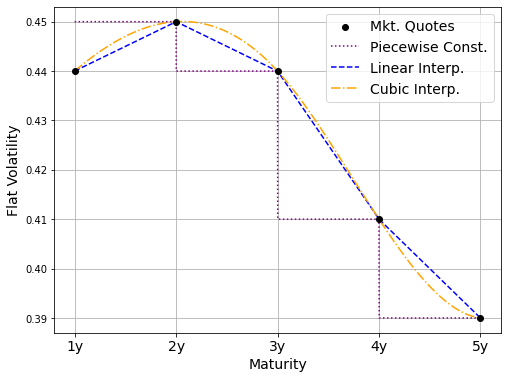
\includegraphics[width=0.6\linewidth]{addons/flat_volatilities}
\end{center}
\label{fig:flat_volatilities}
\end{figure}

Once "estimated" $\sigma^{flat}_{1y6m}$ We will be able to solve a single volatility from previous Equation by using a Newton-Raphson or Brent method.

\item We can apply the same method for the $1y6m$ forward starting caplet to get the volatility, $\sigma^{flat}_{2y}$ is quoted so no interpolation is needed here.
\begin{equation}
\begin{gathered}
\text{Cpl}_{1y6m, 2y}(\sigma^{spot}_{2y})= \text{Cap}_{2y}-\text{Cap}_{1y6m} \\[0.3cm]
\text{Cap}_{2y}(\textcolor{ipython-green}{\sigma^{flat}_{2y}})=\text{Cpl}_{0,6m}(\textcolor{ipython-green}{\sigma^{flat}_{2y}}) + \text{Cpl}_{6m,1y}(\textcolor{ipython-green}{\sigma^{flat}_{2y}}) + \ldots + \text{Cpl}_{1y6m,2y}(\textcolor{ipython-green}{\sigma^{flat}_{2y}}) \\[0.3cm]
\text{Cap}_{1y6m}(\textcolor{ipython-green}{\sigma^{flat}_{1y6m}})=\text{Cpl}_{0,6m}(\textcolor{ipython-green}{\sigma^{flat}_{1y6m}}) + \text{Cpl}_{6m,1y}(\textcolor{ipython-green}{\sigma^{flat}_{1y6m}}) + \text{Cpl}_{1y,1y6m}(\textcolor{ipython-green}{\sigma^{flat}_{1y6m}})
\end{gathered}
\end{equation}

\item Keep iteratively to solve for all the remaining volatilities using the very same technique.
\end{enumerate}
\end{question}
\clearpage

\section{Negative Rates}

The financial crisis, which started in 2007, exposed a lack of trust among counterparties. Since then the incorporation of the probability of default in pricing models has become standard.
This lack of trust in the financial system reduced trading activities and kept the money in the pockets.
To recover trust, the central banks decide to intervene and stimulate the monetary supply and demand by lowering the interest rates.
This decision was expected to encourage investors to borrow money at low rate and invest into the economy, which would push its grow. Since 2008 interest rates have gradually been lowered.

Begin June 2014, the rates set by ECB were negative for the first time (-10 bps). Using negative rates to "inspire" investors is certainly unconventional bu not unprecedented (Switzerland, Sweden and Denmark also report negative rates).

In a negative interest rate environment, the ZCBs, may get values that are higher than one unit of currency. This would imply that the Libor rate would be negative. When the the rate is negative the Black-Scholes pricing equation is not properly defined (the logarithm of a negative quantity...).

Instead of using the Geometric Brownian Motion dynamics, the arithmetic Brownian Motion (ABM), that give rise to negative realizations could, for example be chosen. Such a solution, although straight-forward, has a significant disadvantage, however, as the normal distribution has much flatter tails as compared to a log-normal process.

So instead of completely changing the underlying dynamics, the industrial standard fro dealing with the negativity has become to \emph{shift} the original process.

Caplets can be prices under a negative interest rate environment by an \emph{adaptation} of the underlying dynamics of the Libor rate. The shifted process is defined, as
\begin{equation}
\hat{L_k}(t) = L_k(t) + \theta_k
\end{equation}
The corresponding Black equation becomes
\begin{equation}
	\textbf{Cpl}_k(t_0) = N\tau_k P(t_0, T_k)\left[\hat{L_k}(t_0)\Phi(d_1)-\hat{K}\Phi(d_2)\right] 
\end{equation}
where $\hat{K} = K + \theta_k$.

\begin{figure}[htbp]
\begin{center}
	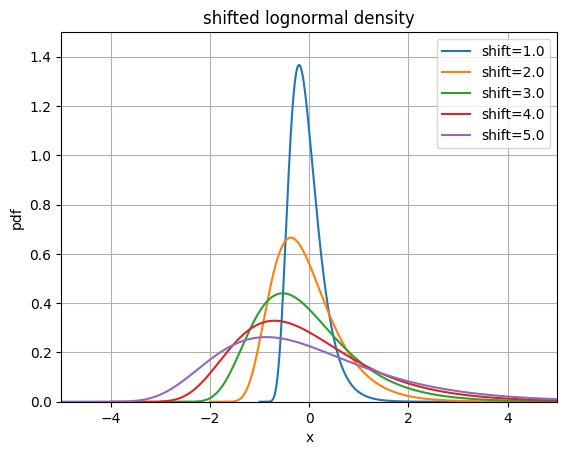
\includegraphics[width=0.6\linewidth]{addons/lognormal_shifted}
\end{center}
\label{fig:lognormal_shifted}
\end{figure}

\begin{question}
Write a python function that simulated shifted-geometric Brownian motion paths.
\end{question}

\begin{question}
Using the function written in the previous exercise, price caplets with Monte Carlo and using Black formula in a regime with negative interest rates. Compare the two results.
\end{question}

\clearpage
\section{Jamshidian Decomposition}
An option on a portfolio of pure discount bonds can be decomposed into a portfolio of options on the individual discount bonds in the portfolio.

Hence, we can think of the European Swaption as a sum of European
options on Zero-Coupon bonds. This method is called Jamshidian’s decomposition, and is mathematically explained as follows:
\begin{equation}
	\max\left[\sum_{i=1}^n C_i p(r, t, s_i) - K, 0\right] = \sum_{i=1}^n C_i \max\left[p(r, t, s_i) - K_i, 0\right]
	\label{eq:jamshidian_decomposition}
\end{equation}

Consider a European Swaption with strike rate $K$, maturity $T$ and nominal $FV$
with payment dates $T_i$ for $i = 1,\ldots, n$. Since the value of a floating rate bond is worth its face value, we can take it as an option on a bond paying $C_i = K_{s_i}$ with strike price $FV$. This option will be exercised when $r(T) < r^*$ where $r^*$ is the solution to
\begin{equation}
	FV = \sum_{i=1}^n C_i p(r^*, T, T_i)
\end{equation}
This means that $FV$ is taken as a sum of discounted flows $C_i$ for a short rate $r^*$ at time $T$. To find the value of $r^*$ we have to discount all the Swap cash-flows, sum them up and let the sum be equal to the notional. We have to use the NewtonRaphson algorithm to follow this calculation $r^*$, that will be the correspondent level of $r$ for that equality to happen. 

Once $r^*$ is found, we have to calculate the discounted cash-flows substituting it in the discounting factor $e^{-r\Delta t}$ and let them be the strike prices of our call options on Swaps.
Afterwards, we calculate the payoff of the call options on the cash-flows with
the strike price mentioned and sum them up. The payoff of this sum of options
will thus be
\begin{equation}
	\max\left[\sum_{i=1}^n C_ip(r, T, T_i)-FV, 0\right]
\end{equation}
which using Eq.~\ref{eq:jamshidian_decomposition} we find is equivalent to
\begin{equation}
	\sum_{i=1}^n C_i \max\left[p(r, T, T_i)-FV_i, 0\right]
\end{equation}
where $FV_i = p(r^*, T, T_i)$. 
Therefore, the Swaption is calculated as the sum of $n$ options on discounted bonds with the exercise price of the $i$th option equal to $FV_i$.

After the price of a European Swaption under the Hull-White model is calculated, we have to calibrate it against the market data. Usually this calibration method is carried out taking the target prices to match the ones given by the Black-76 or Normal-Black models and trying to get as close as possible to them.

\clearpage
\section{Longstaff-Schwartz Algorithm}

Monte Carlo simulation is a flexible and powerful numerical method to value financial derivatives of any kind. However being a forward evolving technique, it is per se not suited to address the valuation of American or Bermudan options which are valued in general by backwards induction. Longstaff-Schwartz provide a numerically efficient method to resolve this problem by what they call \emph{Least-Squares Monte Carlo}.

The problem with Monte Carlo is that the decision to exercise an American option or not is dependent on the \emph{continuation} value. %Consider a simulation with $M+1$ points in time and paths. 
The approach of Longstaff-Schwartz approximates continuation values for American options in the backwards steps by an ordinary least-squares regression.
Equipped with such approximations, the option is exercised if the approximate continuation value is lower than the value of immediate exercise. Otherwise it is not exercised.

\subsection{Bermudan Option}
Consider a bermudan put option with strike $K$ and maturity in $n$ years. Each year you can choose whether to exercise or not.

Let's implement a MC which actually simulates, besides the evolution of the market, what an investor holding this option would do. 

We simulate that 1 year has passed, computing the new value of the asset and of the money market account
\begin{equation}
	\begin{gathered}
		S(t_1=1y) = S(t_0)e^{(r-\frac{1}{2}\sigma^2)(t_1-t_0)+\sigma\sqrt{t_1-t_0}\mathcal{N}(0,1)} \\
		B(t_1=1y)=B(t_0)e^{r(t_1-t_0)}
	\end{gathered}
\end{equation}

At this point the investor could exercise. How does he know if it is convenient? In case of exercise he knows exactly the payoff he's getting. In case he continues, he knows that it is the same of having a European Put Option.

So, in mathematical terms we have the following payoff in 
\begin{equation}
	\max[K-S(t_1), P(t_1,T;S(t_1),K)]
\end{equation}
where $P(t_1,T;S(t_1),K)$ is the price of a Put which can be computed analytically! In the jargon of American products, 
is called the \emph{continuation value}, i.e. the value of holding the option instead of early exercising it.

So the premium of the option is the average of this discounted payoff calculated in each iteration of the Monte Carlo procedure
\begin{equation}
	\cfrac{1}{N}\sum_i\max[K-S(t_1), P(t_1,T;S(t_1),K)]
\end{equation}

We could have priced this product because we have an analytical pricing formula for the put. What if we didn't have it?

Brute force solution: for each realization of $S(t_1)$ we run another Monte Carlo to price the put. This method (called \emph{Nested Monte Carlo}) is very time consuming and quite inefficient, for this very simple case it's time of execution grows as $N^2$, which becomes prohibitive when you deal with more than one exercise date !

Let's search for a finer solution analyzing the relationship between the continuation value and the simulated realization of $S$ at step $t_1$. 

By plotting the discounted payoff at maturity, $P_i$ vs $S_i(T_1)$ (the red line represents the analytical price of the put as a function of $S_i$).

\begin{figure}[htbp]
	\begin{center}
		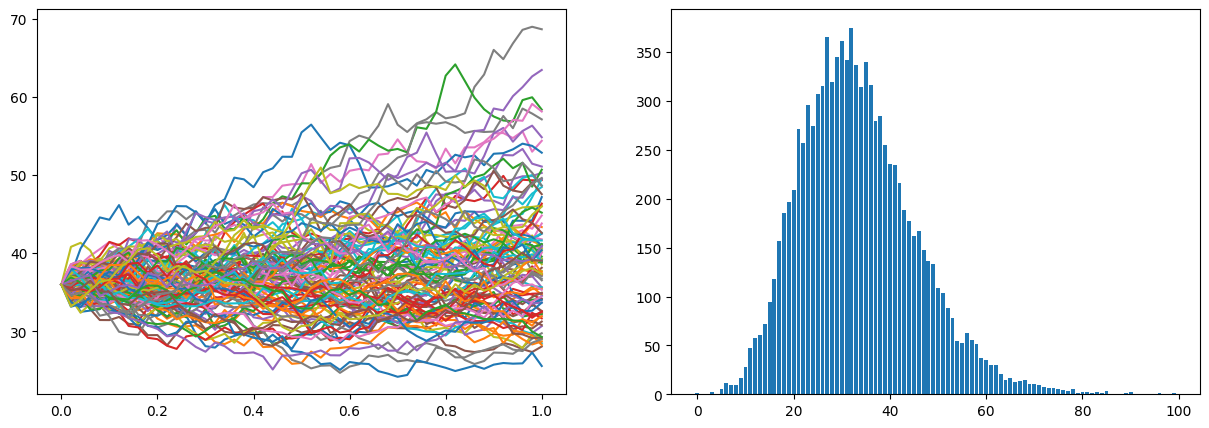
\includegraphics[width=0.8\linewidth]{addons/lsm_paths}
	\end{center}
	\label{fig:lsm_paths}
\end{figure}

The analytical price of the put is a curve which kinds of interpolate the cloud of Monte Carlo points. This suggest us that
\textbf{the price at time $t_1$ can be computed by means of an average on all discounted payoff (i.e. the barycentre of the cloud made of discounted payoff)}.
Which in turn suggest that \textbf{the future value of an option can be seen as the problem of finding the curve that best fits the cloud of discounted payoff up to date of interest.}

As an example in Fig.~\ref{fig:continuation_function} there is a curve found by means of a linear regression on a polynomial of 5th order.

\begin{figure}[htbp]
	\begin{center}
		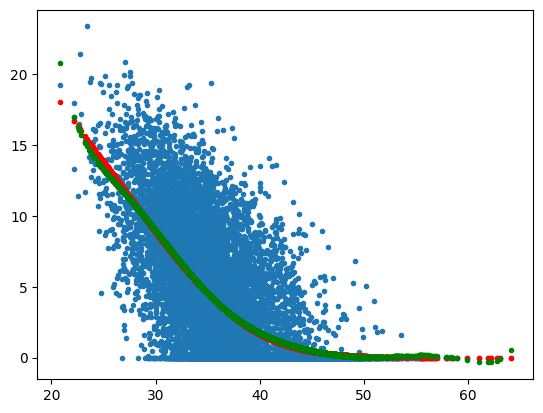
\includegraphics[width=0.5\linewidth]{addons/continuation_function}
	\end{center}
	\label{fig:continuation_function}
\end{figure}

So we have an empirical pricing formula for the put to be used in the Monte Carlo Simulation
\begin{equation}
	P(t_1,T,S(t_1),K)=c_0+c_1 S(t_1) + c_2 S(t_1)^2 + c_3 S(t_1)^3 + c_4 S(t_1)^4 + c_5 S(t_1)^5
\end{equation}

The formula is obviously fast, the cost of the algorithm being just the best fit. Clearly we could have used any form for the curve (not only a polynomial). 

\subsection{The Algorithm}
The major insight of Longstaff-Schwartz is to estimate the continuation value $C_{t,i}$ by ordinary least-squares regression, therefore the name Least Square Monte Carlo for the algorithm. 
They propose to regress the $I$ continuation values $Y_{t,i}$ against the I simulated levels $S_{t,i}$. Given $D$ basis functions $b_i:\mathbb{R}^D\rightarrow\mathcal{R}$ for the regression, the continuation value $C_{t,i}$ is according to the approach approximated by
\begin{equation}
	\hat{C}_{t,i}=\sum_{i=1}^D \alpha^*_{d,t}b_d(S_{t,i})
	\label{eq:continuation_approx}
\end{equation}

The optimal regression parameters $\alpha^*_{d,t}$ are the result of the minimization
\begin{equation}
	\min_{\alpha_{1,t},\ldots,\alpha_{D,t}}\cfrac{1}{I}\sum_{i=1}^I \left(Y_{t,i}-\sum_{i=1}^D\alpha^*_{d,t}b_d(S_{t,i})\right)^2
	\label{eq:optimization_alphas}	
\end{equation}

In some circumstances, the quality of the regression can be improved upon when restricting the paths involved in the regression to those where the option is in-the-money.

\begin{question}
Price an America put option using the LongStaff-Schwartz algorithm. The initial underlying value is $S_0=36$, the volatility is 20\%, the strike price $K=40$, $T=1$, and the risk-free rate 6\% flat.
\end{question}

\begin{question}
Price an Bermudan Swaption using the LongStaff-Schwartz algorithm. %The initial underlying value is $S_0=36$, the volatility is 20\%, the strike price $K=40$, $T=1$, and the risk-free rate 6\% flat.
\end{question}


Let's consider now a generic American product. Here is the Longstaff-Schwartz algorithm
\begin{itemize}
	\item simulate $I$ index level paths with $M+1$ points in time leading to index level values
	\begin{equation*}
		S_{t,i},\quad t \in \{0,\ldots,T\}, i \in \{1,\ldots,I\}
	\end{equation*};
\item for $t=T$ the option value is $V_{T,i}=h_T(S_{T,i})$ by arbitrage arguments;
\item start iterating backwards $t = T-\Delta t, \ldots,\Delta t$:
\begin{itemize}
	\item regress the $T_{t,i}$ against the $S_{t,i}, i\in \{1,\ldots, I\}$, given $D$ basis function $b$;
	\item approximate $C_{t,i}$ by $\hat{C}_{t,i}$ according to Eq.~\ref{eq:continuation_approx} given the optimal parameters $\alpha^*_{d,t}$ from Eq.~\ref{eq:optimization_alphas};
	\item set 
	\begin{equation*}
		V_{t,i}=
		\begin{cases}
			h_t(S_{t,i})\quad\text{if }h_t(S_{t,i})>\hat{C}_{t,i}\text{ exercise takes place}\\
			Y_{t,i}\quad\text{if }h_t(S_{t,i})\leq\hat{C}_{t,i}\text{ exercise does not take place}\\
		\end{cases}
	\end{equation*}
	repeat iteration steps until $t=\Delta t$;
\end{itemize} 
\item for $t=0$ calculate the LSM esitmator
\begin{equation}
	\hat{V}_0^{LSM}=e^{-r\Delta t}\cfrac{1}{I}\sum_{i=1}^{I}V_{\Delta t, i}
\end{equation} 
\end{itemize}

\clearpage
\section{Callable Bond}

When it comes to analyzing callable bonds, investors have a variety of tools and techniques at their disposal. These tools and techniques enable investors to assess the value of callable bonds and make informed investment decisions. In this section, we will discuss some of the most commonly used callable bond analysis tools and techniques.

1. Yield to Call (YTC)

YTC is a measure of the return an investor can expect if a callable bond is called by the issuer. It takes into account the call price, the coupon rate, and the time to call. YTC is an important metric for investors because it allows them to compare the potential return of a callable bond to that of a non-callable bond. However, it is important to note that YTC assumes that the issuer will call the bond at the first opportunity, which may not always be the case.

2. Yield to Worst (YTW)

YTW is a measure of the return an investor can expect if a callable bond is not called by the issuer. It takes into account the yield to maturity and the yield to call, whichever is lower. YTW is important for investors because it provides a more conservative estimate of the potential return of a callable bond. It is also important to note that YTW assumes that the bond will not be called, which may not always be the case.

3. option-Adjusted spread (OAS)

OAS is a measure of the yield spread between a callable bond and a risk-free bond of the same maturity. It takes into account the optionality of the callable bond, which allows the issuer to call the bond at any time. OAS is important for investors because it provides a more accurate estimate of the credit risk associated with a callable bond.

4. Duration

Duration is a measure of the sensitivity of a bond's price to changes in interest rates. It takes into account the bond's cash flows, maturity, and yield. Duration is important for investors because it allows them to assess the risk associated with a callable bond. Callable bonds typically have shorter durations than non-callable bonds, which means that they are less sensitive to changes in interest rates.

5. Monte Carlo Simulation

Monte Carlo simulation is a technique that uses random variables to simulate the potential outcomes of an investment. It takes into account a range of possible interest rate scenarios and calculates the potential return of a callable bond under each scenario. Monte Carlo simulation is important for investors because it allows them to assess the potential risk and return of a callable bond in a variety of market conditions.

A callable bond is a bond in which the issuer reserves the right to redeem the bond at different discrete times, possibly for different redemption values. When a callable bond is bought, no one knows when the bond will be called, however it can nly be called at the times agreed upon at issue.

The most common questions asked with callable bonds involve either

1. determining the maximum price that can be paid for the bond to guarantee a certain yield rate, or
2. detemining the minimum yield rate for a bond that was bought at a certain price.

The recommende strategy for solving callable bond problems is to crete a two column table with the first represeint ghe timme at which the bond can be called.

For type 1. problems, the second column is the corresponding price in order to receive the desired yield rate, keeping in mind the redemption value may be different at the different redemption dates. Then think through what happens whine the bond is bought for the prices in the table but redeemed at other times in the table, an answer the question accrodgingly.

For type 2. rpboems the second column of the table is the yield rate tha would produce the given price, again keeping in mind the redemption value may be different at the different edemption dates.



Bonds with European call option just have a single possible call date. Let's denote the call date by $t_c$ and the notice time as $t_n$. Also, we denote the call price with $X$. 

In general, we can assume that \textbf{it is optimal for the issuer to minimize the value of the contract}. It means the issuer will exercise the option if the price of the callable bond exceeds the exercise price at the notice date. Otherwise, she will give up the option right and the callable bond price is equal to that of the non-option bond.

Denote by $r_b$ the \emph{break-even} interest rate which represents the rate value such that the issuer is indifferent between exercising the option or not.

It can be calculated by,
\begin{equation}
X\cdot D(t_n, t_c) - P(r,t_n)=0
\end{equation}
where $D(t_n, t_c)$ is the discount factor between notice and exercise dates and $P(r,t_n)$ the price of the callable bond an instant before the notice date.

We know the value of the callable bond $P(r,t_n)$ since it is equal to the value of the non-option bond. The solution of equation is the cross point between the two curves.

\begin{figure}[htbp]
	\begin{center}
		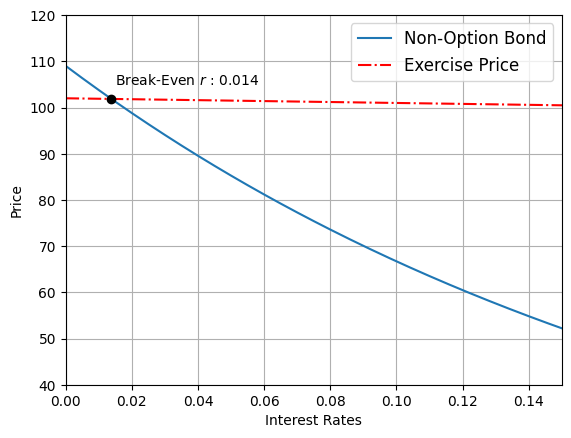
\includegraphics[width=0.5\linewidth]{addons/callable_bond}
	\end{center}
	\label{fig:callable_bond}
\end{figure}


\begin{question} A 1000 face value 20-years callable bond with 5\% annual coupons is selling 1150. The bond can be redeemed at the end of 18 years for 950, at the end of 19 years for 975, or at the end of 20 years for 1000. Determine the minimum annual yield rate that a buyer will earn on this bond.
\end{question}
%\begin{solution}
%	3.647\%
%	
%	18 3.831\%
%	19 3.87\%
%	20 3.91\%
%	
%	
%\end{solution}

\begin{question} A 1000 face value 20-year callable bond with 3\% annual coupons can be redeemed according to the following schedule:
\begin{itemize}
	\item 1000 at the end of years 10 through 14;
	\item 1075 at the end of years 15 through 17;
	\item 1125 at the end of years 18 through 20.
\end{itemize}
Determine the maximum price a buyer should pay in order to earn an annual yield of at least 5\%.
\end{question}
%\begin{solution}
%	def ytm(y, c, t, f, red):
%	...:     val = sum([c*f/(1+y)**k for k in range(1, t+1)])
%	...:     return val + red/(1+y)**t
%	...: 
%	
%	In [28]: ytm(0.05, 0.03, 10, 1000)
%	
%	10 845.57
%	11 833.87
%	NOTE: The prices will systematically increase or decrease (decrease in this problem) when the redemption value remains the same.
%	Therefore, we only need to check endpoints for the same redemption values.
%	14 802.03
%	15 828.48
%	17 807.24
%	18 818.15
%	20 797.87 which is the answer
%	
%	Imagine you bought the bond for 797.87. Determine the yield if the bond is redeemed at the end of year 16.
%	
%	In [51]: def find_ytm(y, c, t, f, red, price):
%	...:     val = sum([c*f/(1+y)**k for k in range(1, t+1)])
%	...:     return val + red/(1+y)**t - price
%	
%	n [55]: brentq(find_ytm, 0, 0.1, args=(0.03, 16, 1000, 1075, 797.87))
%	Out[55]: 0.05204043575983794
%	
%\end{solution}

\begin{question} A 1000 face value 10-year callable bond with 8\% semiannual coupons is bought for 1050.  The bond can be redeemed at the end of any year starting with year 7.  Determine the minimum annual yield for this bond.
\end{question}
%\begin{solution}
%	In [70]: def b_ytm(price, fv, call_price, T, coup, freq=2, guess=0):
%	...:     freq = float(freq)
%	...:     periods = T*freq
%	...:     coupon = coup*fv/freq
%	...:     dt = [(i+1)/freq for i in range(int(periods))]
%	...:     ytm_func = lambda y: sum([coupon/(1+y/freq)**(freq*t) for t in dt]) + fv/(1+y/freq)**(freq*max(dt)) - price
%	...:     return newton(ytm_func, guess)
%	
%	There is no redemption value stated or implied. For all bond problems, when this is the case, assume the bond is redeemable at par. 
%	14 3.54\%
%	16 3.58\%
%	18 3.62\%
%	20 3.64\%
%	NOTE: The interest rates will systematically increase or decrease (increase in this problem) when the redemption value remains the same. Therefore, we only need to check endpoints for the same redemption values.
%\end{solution}

\begin{question} A 1000 face value 20-years callable bong, reddeemable at 1200, with 5\% annual coupons can be redeemed at the end of year 18, 19, 20. Determine the maximum price a buyer is willing to pay in order to earn an annual yield of at least 3\%
\end{question}
%1392.55
%In [116]: price(1000, 1200, 19, 0.05, 0.03, 1)
%Out[116]: 1286.475982125383
%
%In [117]: price(1000, 1200, 18, 0.05, 0.03, 1)
%Out[117]: 1275.0702615891446
%
%In [118]: price(1000, 1200, 20, 0.05, 0.03, 1)
%Out[118]: 1297.5494972091096


\begin{question} A 1000 face value 20-years callable bond with 4\% annual coupons can be redeemed according to the following schedule:
1000 at end 12-14, 1025 at end 15-17, 975 at end 18-20.
Determine the maximum price a buyer is willing to pay in order to earn an annual yield of at least 4\%
987.66
\end{question}

\begin{question} A 1000 face value 10\% annual coupon bond is redeemable as follows: 1100 at 15, 16,17, 1000 at 18,19,20. A buyer pays 1500 for this bond, Determine the buyer minimum annual yield.
\end{question}
%In [70]: def b_ytm(price, fv, call_price, T, coup, freq=2, guess=0):
%...:     freq = float(freq)
%...:     periods = T*freq
%...:     coupon = coup*fv/freq
%...:     dt = [(i+1)/freq for i in range(int(periods))]
%...:     ytm_func = lambda y: sum([coupon/(1+y/freq)**(freq*t) for t in dt]) + fv/(1+y/freq)**(freq*max(dt)) - price
%...:     return newton(ytm_func, guess)
%5.474%
%In [96]: b_ytm(1500, 1000, 1100, 15, 0.1, 1)
%Out[96]: 0.051378853239277274
%
%In [97]: b_ytm(1500, 1000, 1100, 16, 0.1, 1)
%Out[97]: 0.05290592139352415
%
%In [98]: b_ytm(1500, 1000, 1100, 17, 0.1, 1)
%Out[98]: 0.05423627236846406
%
%In [99]: b_ytm(1500, 1000, 1000, 18, 0.1, 1)
%Out[99]: 0.05540277776325789
%
%In [100]: b_ytm(1500, 1000, 1000, 19, 0.1, 1)
%Out[100]: 0.05643146238150476
%
%In [101]: b_ytm(1500, 1000, 1000, 20, 0.1, 1)
%Out[101]: 0.05734319789419295

\begin{question} A 20-year 10\% 1000 bond that pays interest half-yearly is redeemable (callable) in twelve years at a buy-back (call) price of 1150. The bond's current yield to maturity is 9.50\% annually. You are required to determine 
\begin{enumerate}[label=(\alph*),font=\itshape]
	\item the yield to call;
	\item the yield to call if the buy-back price is only 1100;
	\item the yield to call if instead of twelve years the bond can be called in eight years, the buy-back price being 1150.
\end{enumerate}
\end{question}
%\begin{solution}
%	
%	def price(y, c, t, f, red):
%	...:     val = sum([c*f/(1+y)**k for k in range(1, t+1)])
%	...:     return val + red/(1+y)**t
%	
%	def price(fv, call_price, T, coup, y, freq=2):
%	freq = float(freq)
%	periods = T*freq
%	coupon = coup*fv/freq
%	dt = [(i+1)/freq for i in range(int(periods))]
%	return sum([coupon/(1+y/freq)**(freq*t) for t in dt]) + fv/(1+y/freq)**(freq*max(dt)) 
%	
%	A callable bond is a debenture issued with a call provision, in which this bond can be redeemed earlier than its initial maturity. The call price is determined at the issuance.
%	
%	Given the number of periods $N$, the par 1000, the semiannual coupon = $1000\cdot 0.1 \cdot 0.5 = 50$, and the semiannual yield $I=0.0475$ determine the current price of the bond
%	\begin{equation*}
%		P_0 = coupon \frac{1-(1+I)^{-N}}{I} + \frac{Par}{(1+I)^N} = 50 \frac{1-(1+0.0475)^{-40}}{0.0475}+\cfrac{1000}{(1+0.0475)^40} = 1044.41
%	\end{equation*}
%	\begin{enumerate}[label=(\alph*),font=\itshape]
%		\item To determine the yield to call if the price is 1150, 
%		FV = 1,150
%		PV = 1,044.41
%		PMT = 50
%		N = 12 x 2 = 24
%		CPT I = 5.01
%		YTC = 5.01% x 2 = 10.02%
%		\item Determine the yield to call if the call price is Rs 1,100; using the financial calculator:
%		
%		FV = 1,100
%		PV = 1,044.41
%		PMT = 50
%		N = 12 x 2 = 24
%		CPT I = 4.91
%		YTC = 4.91% x 2 = 9.82%
%		\item Determine the yield to call if the call price is Rs 1,150; and this bond will be called in 8 yearsl of ; using the financial calculator:
%		
%		FV = 1,150
%		PV = 1,044.41
%		PMT = 50
%		N = 8 x 2 = 16
%		CPT I = 5.21
%		YTC = 5.21% x 2 = 10.42%
%	\end{solution}


\clearpage
\section{Reverse Floater}

* For instance, in September 2009, the short-term interest rate, the 3-month EURIBOR, **was at 0.5%**, and the forward curve was rising rather steeply, i.e. the implied forward 3-month EURIBOR in 3 years **was at 3.3%**. 
* The 3-year interest rate for a fixed-coupon bond **was at 3.5%** at the time. 
* It was possible to construct a 3-year reverse floater bond paying:

$$ 6\% - 2 \cdot \text{3M-EURIBOR}$$

(the coupon payments usually occur on a quarterly basis). 
* Should the 3-Month EURIBOR not move during the first year, the coupon would amount to $6\% - 2 \cdot 0.5\% = 5\%$. 
* Compared to a floating rate bond, the outperformance would be 4.5% for that period. 
%* After 3 years, the invested nominal is redeemed along with the last coupon.

Vega 

$$V_{\text{cap}}=F\Phi(d_1) - K\Phi(d_2)$$

$$\nu = \frac{\partial V_{\text{cap}}}{\partial\sigma} =
F\phi(d_1)$$

\begin{figure}[htbp]
	\begin{center}
		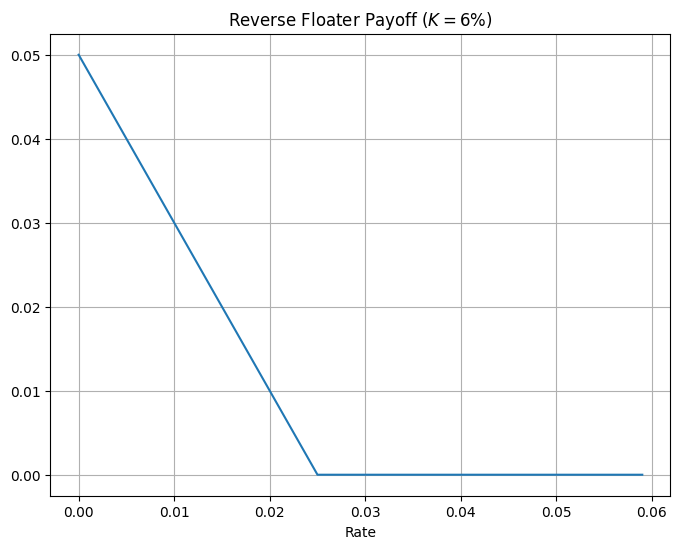
\includegraphics[width=0.5\linewidth]{addons/reverse_floater_payoff}
	\end{center}
	\label{fig:reverse_floater_payoff}
\end{figure}

\begin{figure}[htbp]
	\begin{center}
		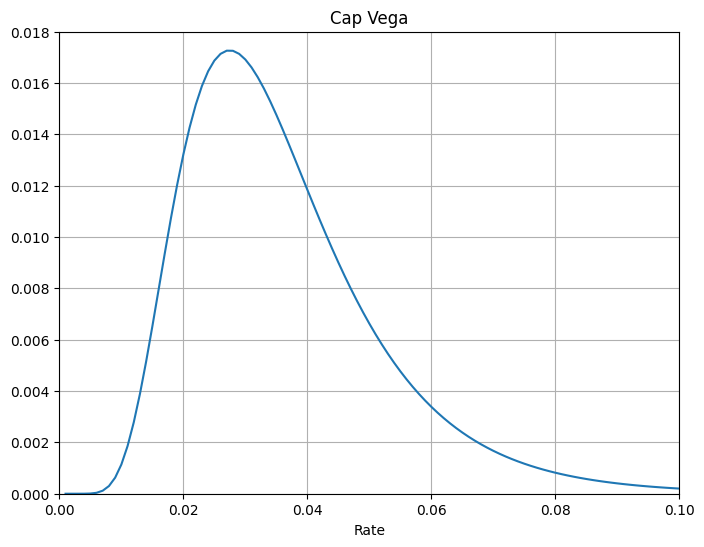
\includegraphics[width=0.5\linewidth]{addons/cap_vega}
	\end{center}
	\label{fig:cap_vega}
\end{figure}

\clearpage
\section{Girsanov Theorem}
Let’s start with a standard Brownian motion $W_t^{\mathcal{P}} = \mathcal{N}_{\mathcal{P}}(0,t)$ under a probability measure $\mathcal{P}$, and adapted to a filtration $\mathcal{F}_t$. In Fig.~\ref{fig:brownian_motion_nodrift} 30 simulated path evolutions of $W_t^{\mathcal{P}}$ are shown, as expected there is no drift.
	
\begin{figure}[htbp]
	\begin{center}
		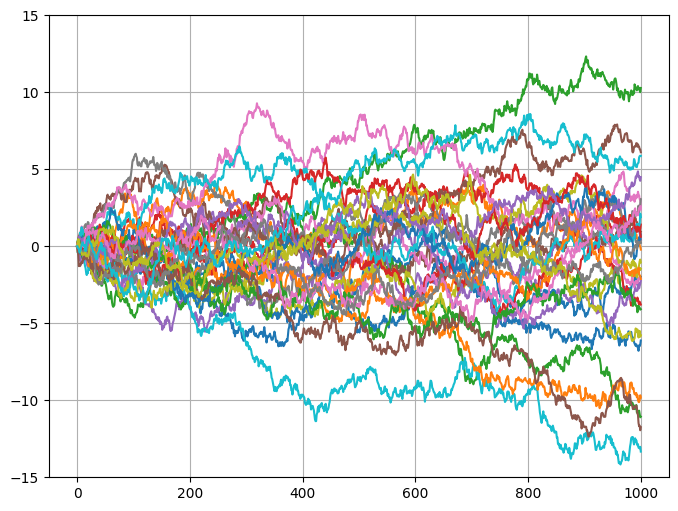
\includegraphics[width=0.5\linewidth]{addons/brownian_motion_nodrift}
	\end{center}
	\label{fig:brownian_motion_nodrift}
	\caption{Thirty realization of the simple Brownian motion $W_t^{\mathcal{P}}$.}
\end{figure}

For exemplification, let us now construct a "drifty" process $Y_t=\mu t+\sigma W_t^{\mathcal{P}}\in \mathcal{N}_{\mathcal{P}}(\mu t, \sigma^2 t)$, that is a Wiener process with drift $\mu$ and diffusion $\sigma$; in other words, $\mathbb{E}^{\mathcal{P}}[Y_t]=\mu t$ and $\text{Var}^{\mathbb{P}}[Y_t]=\mathbb{E}^{\mathcal{P}}[Y^2_t]-\mathbb{E}^{\mathcal{P}}[Y_t]^2=\sigma^2 t$.

%Incidentally, note the terminology: the drift is not an expectation, but rather the rate of change in expectation, and the diffusion is not a standard deviation, but rather the square root of the rate of change in variance. 
Figure~\ref{fig:brownian_motion_drift} shows 30 simulated paths for the evolution of $Y_t$ ($\mu = 0.8$ and $\sigma =1.25$). There the drift is visually apparent.
\begin{figure}[htbp]
\begin{center}
	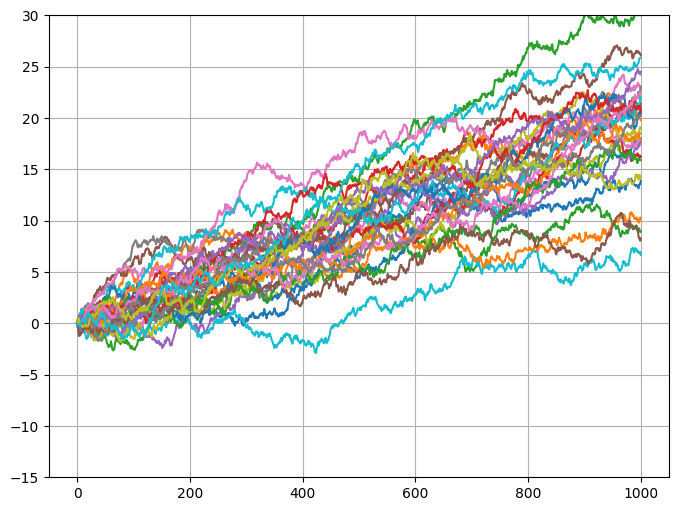
\includegraphics[width=0.5\linewidth]{addons/brownian_motion_drift}
\end{center}
\label{fig:brownian_motion_drift}
	\caption{Thirty realization of the "drifty" Brownian motion $Y_t$.}
\end{figure}

We aim at applying a change of measure from $\mathcal{P}$ into a new probability $\mathcal{Q}$, such that $Y_t$ becomes driftless (a martingale) under $\mathcal{Q}: \mathbb{E}^{\mathcal{Q}}[Y_t]=0$, yet with the same diffusion as under $\mathcal{P}$: $\text{Var}^{\mathcal{Q}}[Y_t]=\sigma^2 t$

Let $\mu^{*}$ be a new drift and assume $\\gamma_t = \frac{\mu_t^{*}-\mu_t}{\sigma_t}$. According to the Girsanov Theorem the process
\begin{equation}
dW^{*}_t = -\gamma_t dt + dW_t
\end{equation}
is a Brownian motion under the new measure $\mathcal{Q}$, equivalent to $\mathcal{P}$, is defined by the Radon-Nikodym derivative
\begin{equation}
\cfrac{d\mathcal{Q}}{d\mathcal{P}} = \exp\left(-\frac{1}{2}\int_0^t\gamma_s^2 ds + \int_0^t\gamma_s dW_s\right)
\end{equation}

\begin{question}
Consider a Wiener process with drift $\mu=0.05$ and diffusion coefficient $\sigma=0.2$. Determine the appropriate transformation, according to the Girsanov Theorem which makes the original process driftless. Verify that applying the Radon-Nikodym to the a simulated path of the process the drift indeed disappear.

\begin{figure}[htbp]
	\begin{center}
		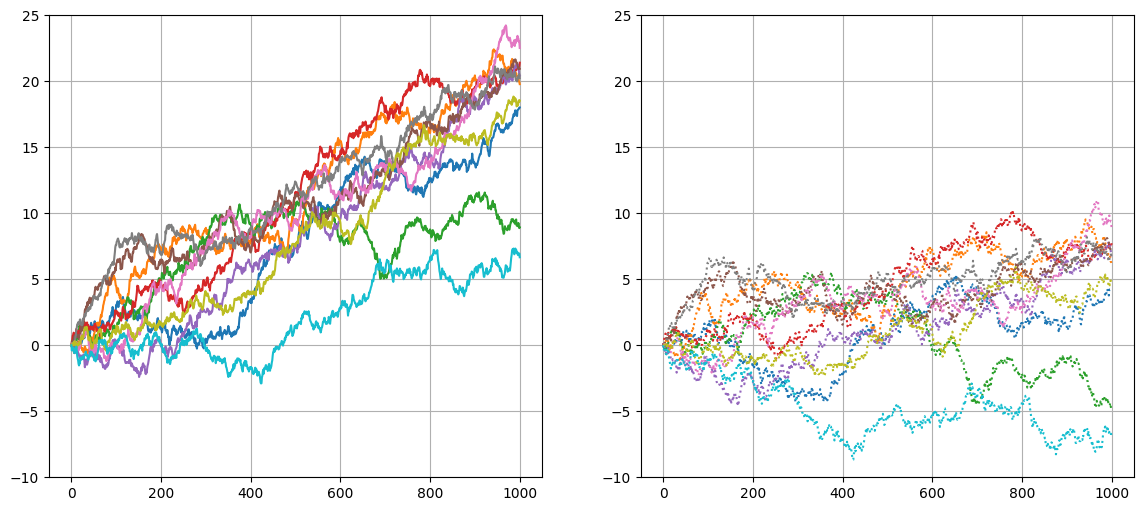
\includegraphics[width=0.5\linewidth]{addons/brownian_motion_girsanov}
	\end{center}
	\label{fig:brownian_motion_girsanov}
\end{figure}
\end{question}

\begin{question}
Given an underlying asset $S$ which currently is valued 100 simulate $N$ possible realization of the random variable $S$ both under the \emph{physical} probability measure and the 
and a 1 year call option on that asset with strike $K=120$ determine 

Other  Consider a Wiener process with drift $\mu=0.05$ and diffusion coefficient $\sigma=0.2$. Determine the appropriate transformation, according to the Girsanov Theorem which makes the original process driftless. Verify that applying the Radon-Nikodym to the a simulated path of the process the drift indeed disappear.

mu = 0.05
r = 0.01
sigma = 0.20
l = (mu-r)/sigma
S0 = 100
K = 120
T = 1
M = 252
dt = T/M
N = 10000
\begin{figure}[htbp]
	\begin{center}
		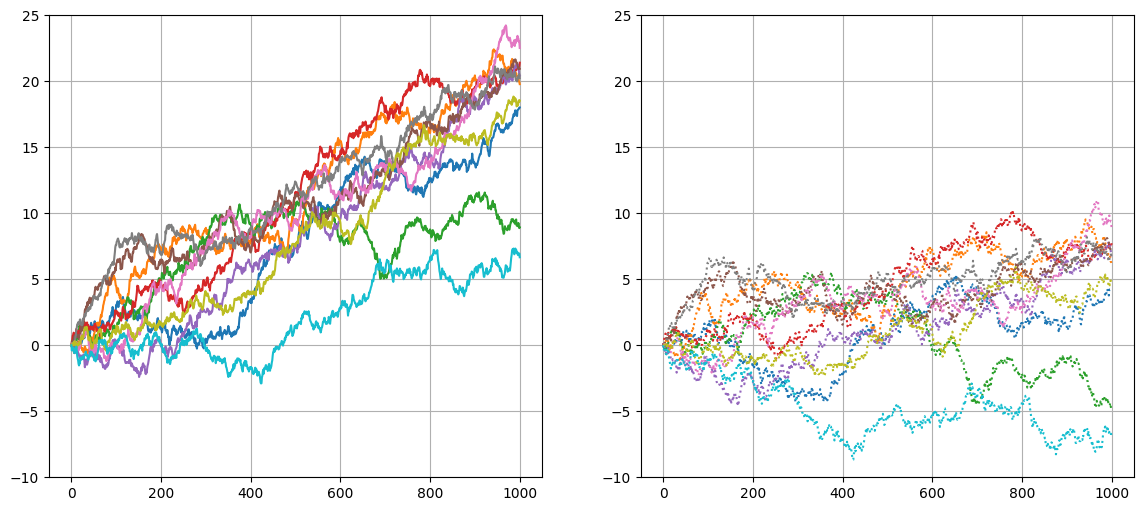
\includegraphics[width=0.5\linewidth]{addons/brownian_motion_girsanov}
	\end{center}
	\label{fig:brownian_motion_girsanov}
\end{figure}
\end{question}

\clearpage
\section{Importance Sampling}
Assume we want to calculate the expectation $\mathbb{E}[f(X)]$
\begin{equation}
\mathbb{E}[f(X)] = \int_{-\infty}^\infty f(x)p(x)dx
\end{equation}
where $p(x)$ is the probability density function associated to the random variable $X$.

We can approximate this expectation using numerical approximation, i.e. Monte Carlo simulation, by sampling $n$ random values from the distribution $p$ and then calculating the sample mean as:
\begin{equation}
\bar{f}(x) = \frac{1}{n}\sum_i f(x_i)
\end{equation}

The idea behind \textbf{importance sampling} is to use a simple re-formulation trick and write the expectation in a slightly different form
\begin{equation}
\mathbb{E}[f(X)] = \int_{-\infty}^\infty f(x)\frac{p(x)}{q(x)}q(x)dx
\end{equation}
giving the expectation of $f(x)\frac{p(x)}{q(x)}$ over the distribution $q$. And with that, allowing us to calculate the sample mean by sampling from $q$:
\begin{equation}
\bar{f}(x) = \frac{1}{n}\sum_i f(x_i)\frac{p(x)}{q(x)}
\label{eq:reformulated_expectation}
\end{equation}

\subsection{Variance Reduction}
From probability theory we know that the variance of the standard Monte Carlo estimator is given by:
\begin{equation}
\cfrac{1}{n}\cdot\text{Var}[f(x)] = \cfrac{1}{n}\cdot\mathbb{E}[(f(X)-\mathbb{E}[f(X)])^2]
\end{equation}

Hence the variance for the re-formulated importance sampling estimator in Eq.~\ref{eq:reformulated_expectation} is:
\begin{equation}
\cfrac{1}{n}\cdot\text{Var}\left[\cfrac{p(x)}{q(x)}f(x)\right]
\end{equation}

This give us a hint on how to find a way to reduce the variance. And indeed it is relatively easy to see that this variance could be reduced to 0 by choosing $q$ as:
\begin{equation}
\begin{aligned}
q(x)&=\cfrac{f(X)p(x)}{\mathbb{E}[f(X)]} \implies \cfrac{1}{n}\cdot\text{Var}[\mathbb{E}[f(X)]] = \cfrac{1}{n}\cdot\mathbb{E}[(\mathbb{E}[f(X)]-\mathbb{E}[\mathbb{E}[f(X)]])^2]=\\
&=\cfrac{1}{n}\cdot\mathbb{E}[(\mathbb{E}[f(X)]-\mathbb{E}[f(X)])^2] = 0
\end{aligned}
\end{equation}

Naturally, we don’t know $\mathbb{E}[f(X)]$, as the reason we are doing this sampling after all is to find the expectation of $f$.
However, we can think of the denominator of the previous expression as some normalisation constant, and consider to construct $q$ such that it has \textbf{high} density wherever $f(x)p(x)$ is \textbf{high}.

\subsection{Practical Example}
For the sake of demonstration, we choose $f=\mathcal{N}(5, 1)$, and the probability distribution $p=\mathcal{N}(9,2)$ which do not overlap too well, see Fig.~\ref{fig:f_and_p}.
\begin{figure}[htbp]
\begin{center}
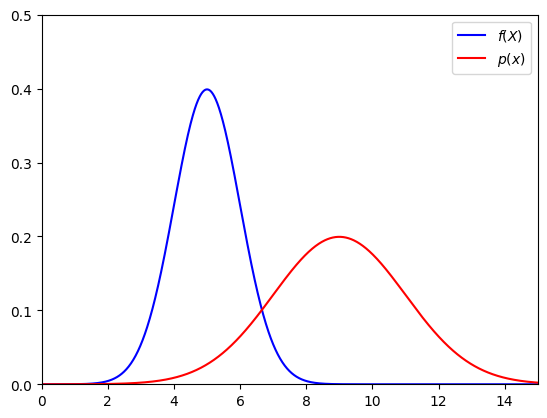
\includegraphics[width=0.5\linewidth]{addons/f_and_p}
\end{center}
\label{fig:f_and_p}
\end{figure}

To approximate numerically the expectation, as stated above, we would now sample values $x_i$ from the distribution $p$, and compute the mean of $f(x_i)$.

Intuitively one can see why sampling from this distribution is a bad idea: for most values sampled from $p$, $f$ will be close to 0, but for a few sampled values $f$ will be very large, thus we obtain a large variance.

\begin{figure}[htbp]
\begin{center}
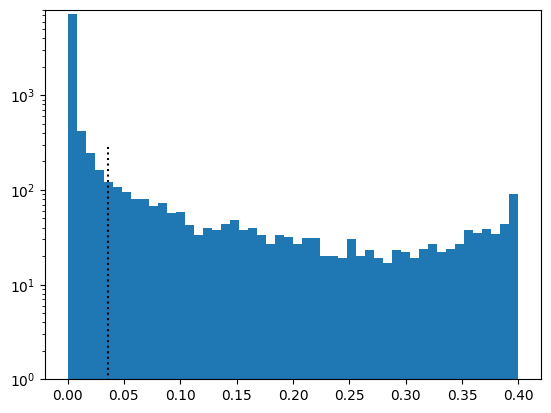
\includegraphics[width=0.5\linewidth]{addons/bad_sampling}
\end{center}
\label{fig:bad_sampling}
\end{figure}

Looking at Fig.~\ref{fig:bad_sampling} it is apparent how the vast majority of samples piles up at 0 (notice the logarithmic scale of the plot). 
Therefore, as outlined above, to make the sampling more efficient, we can try a new distribution $q = \mathcal{N}(5.8, 1)$, which satisfies the criterion that its pdf is high in regions where $f(x)p(x)$ is high, see Fig.~\ref{fig:fp_and_q}.

\begin{figure}[htbp]
\begin{center}
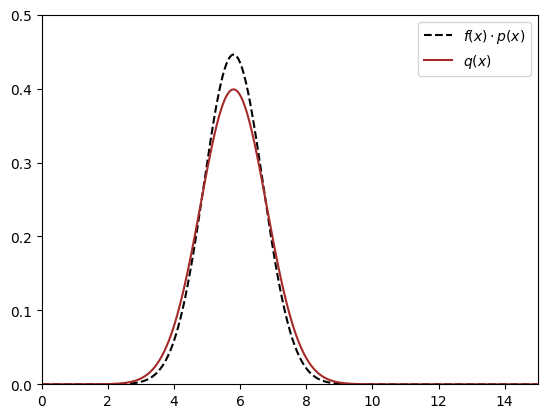
\includegraphics[width=0.4\linewidth]{addons/fp_and_q}
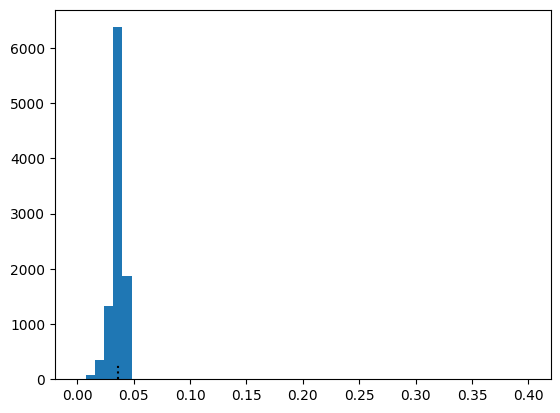
\includegraphics[width=0.4\linewidth]{addons/good_sampling}
\end{center}
\label{fig:fp_and_q}
\end{figure}

The resulting sampling is much better since the values are now clustered around 0.03. Comparing the estimates of the expectation in the two cases shows that the value is essentially the same, but the variance almost a factor 200 lower when using the importance sampling.
\begin{ioutput}
Numerical Simulation: mean 0.03611, variance 0.00759
Importance Sampling: mean 0.03603, variance 0.00003
\end{ioutput}
Note that in general it’s not trivial at all to find $q$, and certainly there are much more difficult real-word scenarios. For this example I actually plotted $p(x)f(x)$ and then picked a $q$ which resembled it best.

\begin{question}
Implement the importance sampling example outlined above, trying to reproduce the results quoted in the text.
\end{question}
\begin{question}
Estimate how unlucky is a 25 standard deviation return
\begin{equation*}
\theta := P(X\geq 25) = \mathbb{E}[\mathbbm{1}_{X\geq 25}]  \quad\text{where } X\sim \mathcal{N}(0, 1)
\end{equation*}
\end{question}
\begin{question}
Consider a one year ($T=1$) call option with $S_0=100$ , $K=170$,  $\sigma=0.2$, and $r=0.06$. The option is far out of the money, assuming we need to estimate its value using Monte Carlo simulation, improve the efficiency of the calculation with importance sampling.

\noindent
Interesting reference \emph{Variance Reduction Techniques of Importance Sampling Monte Carlo Methods for Pricing Options}, 
Journal of Mathematical Finance, 2013, 3, 431-436.
\end{question}

\clearpage
\tableofcontents
\end{document}
